\chapter{Rejestry}

\section{Rejestr szeregowy (przesuwający)}

\begin{itemize}
    \item Należało przetestować działanie rejestru szeregowego korzystając z układu 74164. (\ref{link:74164})
        \begin{figure}[H]
            \centering
            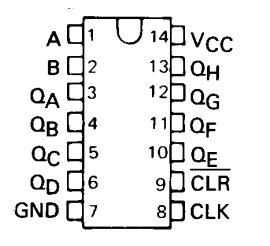
\includegraphics[width=0.5\textwidth]{img/schemes/74164_pins.png}
            \caption{Piny TTL 74164}
            \label{rejestr_szeregowy:piny}
        \end{figure}
    \item Korzystając impulsatorów podajemy wartości na wejście A oraz B rejestru szeregowego.
    \item Wejście zegara (pin 8) obsługujemy za pomocą generatora funkcyjnego generującego sygnał o zadanych wartościach:
        \begin{center}
            f = 1Hz \\
            $U_{low}$ = 0V \\
            $U_{high}$ = 5V
        \end{center}
    \item Wyjścia rejestru QA-QH (piny 3,4,5,6,10,11,12,13) zostały wyprowadzone do diod elektroluminescencyjnych znajdujących się na prawej stronie płytki.
        \begin{figure}[H]
            \centering
            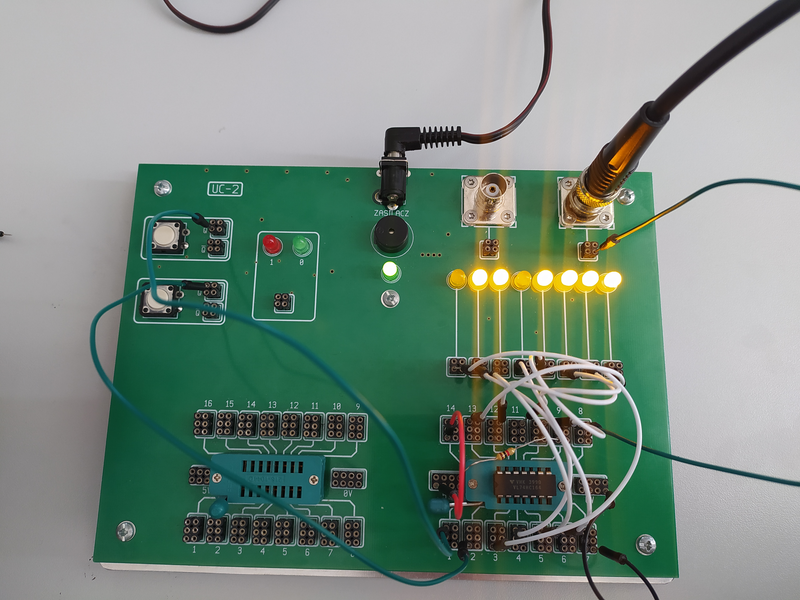
\includegraphics[width=0.7\textwidth]{img/74164/1653500524524_scaled.png}
            \caption{Zbudowany rejestr szeregowy}
            \label{rejestr_szeregowy:zbudowany}
        \end{figure}
        
        \begin{figure}[H]
            \centering
            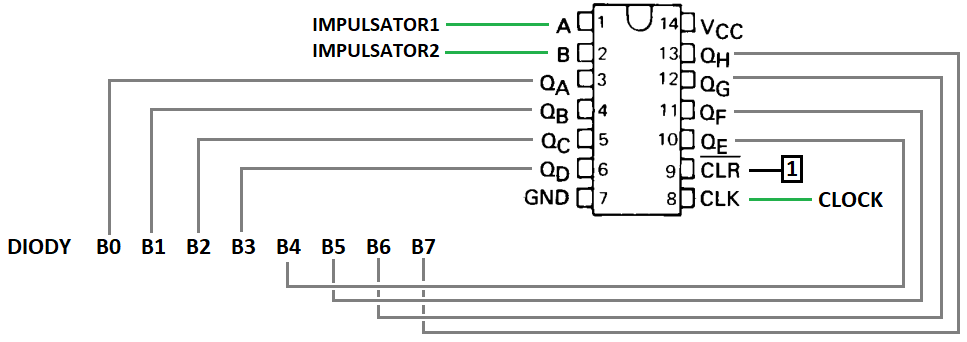
\includegraphics[width=\textwidth]{img/schemes_w_pins/74164_w_pins.png}
            \caption{Schemat z połączonymi pinami}
            \label{rejestr_szeregowy:schemat_z_pinami}
        \end{figure}
        
    \item Podczas jednoczesnego wysłania impulsu z impulsatora 1 oraz 2 (wejścia A, B) na rejestrze pojawia się logiczna 1, która przesuwa się do kolejnej pozycji razem z każdym tyknięciem zegara.
    \item Zbudowany rejestr szeregowy działał \textbf{poprawnie}.
\end{itemize}

\pagebreak

\section{Rejestr równoległy (buforowy)}

\begin{itemize}
    \item Należało przetestować działanie rejestru równoległego korzystając z układu 74165. (\ref{link:74165})
        \begin{figure}[H]
            \centering
            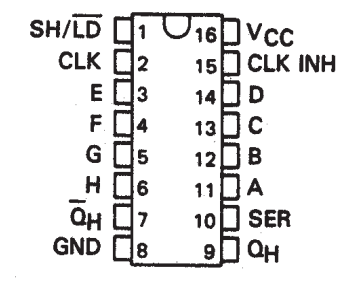
\includegraphics[width=0.5\textwidth]{img/schemes/74165_pins.png}
            \caption{Piny TTL 74165}
            \label{rejestr_rownolegly:piny}
        \end{figure}
    \item Korzystając impulsatorów podano wartości na 2 z 8 pinów wejściowych (B oraz C).
    \item Wejście zegara (pin 8) obsługujemy za pomocą generatora funkcyjnego generującego sygnał o zadanych wartościach:
        \begin{center}
            f = 1Hz \\
            $U_{low}$ = 0V \\
            $U_{high}$ = 5V
        \end{center}
    \item Wyjście rejestru QH zostało wyprowadzone do testera logicznego.
    \item Wejście SH/LD – wejście sterujące ładowaniem danych lub przesuwaniem informacji w rejestrze. \\
        W stanie niskim do przerzutników rejestru zostaje zapisana informacja z wejść danych A...H. \\ 
        W stanie wysokim informacja w rejestrze może być przesuwana. \\
        \textbf{Do wejścia zostało podpięte logiczne 0 (stan niski).}
    \item Wejście CLK INH – w stanie wysokim blokuje sygnał zegarowy, informacja nie jest przesuwana w rejestrze. \\
        \textbf{Do wejścia zostało podpięte logiczne 0 (stan niski).}
        \begin{figure}[H]
            \centering
            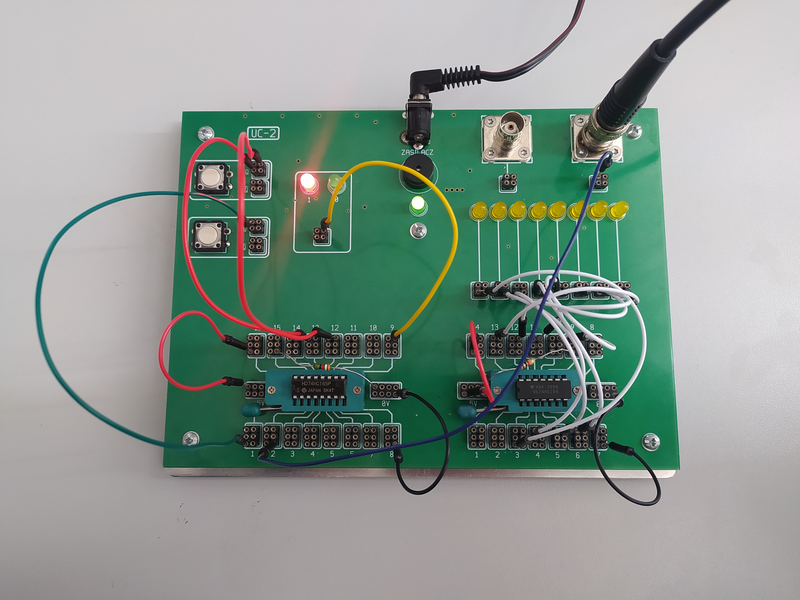
\includegraphics[width=0.7\textwidth]{img/74165/1653500524502_scaled.png}
            \caption{Zbudowany rejestr równoległy}
            \label{rejestr_rownolegly:zbudowany}
        \end{figure}
        
        \begin{figure}[H]
            \centering
            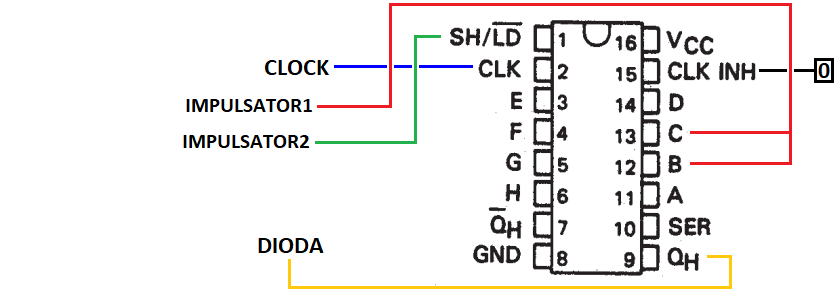
\includegraphics[width=\textwidth]{img/schemes_w_pins/74165_w_pins.png}
            \caption{Schemat z połączonymi pinami}
            \label{rejestr_rownolegly:schemat_z_pinami}
        \end{figure}
        
    \item Z każdym taktem zegara wyświetlany był aktualny bit na rejestrze, po czym wyświetlany był następny bit w rejestrze.
    \item Zbudowany rejestr szeregowy działał \textbf{poprawnie}.
\end{itemize}